\documentclass[a4paper]{article}
\usepackage{graphicx} 
\usepackage[margin=0.5in]{geometry}
\usepackage{amsmath, booktabs, float, hyperref, graphicx}

\title{Milwaukee Bucks Proposal}
\author{Salvin Chowdhury \& Mathias Galvan}
\date{\today}

\begin{document}

\maketitle

\newpage

\section{Proposal Requirements}
The requirements for the project proposal is that it must be 1 page long, and must be approved by the instructor. The
limit is up to groups of three. The proposal must have the following detailed:
\begin{itemize}
    \item Identificaiton of the dataset, including the details as well as what kinds of features are there
    \item Objectives for analyzing the dataset, such as identiying the research question
    \item Displaying the first ten records of the dataset demonstrating that the dataset can be loaded
\end{itemize}

\section{Milwaukee Bucks Dataset}
The dataset to be utilized is the one provided by the Milwaukee Bucks. There are three different datasets, which are
named \texttt{AccountLevel.xlsx}, \texttt{GameLevel.xlsx} and \texttt{SeatLevel.xlsx}. Each dataset will be discussed
in more detail below:

\begin{itemize}
    \item \texttt{AccountLevel}: this dataset provides details about the accounts of the fans, and this contains 
    information such as the account number, number of single game, partial plan or group tickets, as well as basketball
    propensity, number of games the fan has attended and other key information.
    \item \texttt{GameLevel}: this dataset provides details about the games that the Milwaukee Bucks have played in,
    and this contains information such as the the teams that were played against, and if any of those games had a 
    giveaway event.
    \item \texttt{SeatLevel}: this dataset contains information about the level of the game that was attended by the
    fans, the season in which the game was played as well as the tier of the game.
\end{itemize}

\section{Objectives for Analysis}
Using this dataset, the Milwaukee Bucks are considering the introduction of four themed partial ticket plans for the
upcoming season:
\begin{itemize}
    \setlength{\itemsep}{0.2em} 
    \item \textbf{Value Plan}: focuses on affordable tickets for weekday games
    \item \textbf{Marquee Plan Opponent Plan}: featuring games against high-profile opponents
    \item \textbf{Weekend Plan}: highlighting weekend games for fans looking for weekend entertainment
    \item \textbf{Promotional Giveaway Inclusive Plan}: centered around games with promotional giveaways 
\end{itemize}

\noindent These plans are aimed to cater to the diverse fan interests and purchase behaviors. The challenge is to 
leverage the historical ticketing data to predict the likelihood that a account will purchase one of the new partial
plans and which plans the fans are most likely to purchase. \\

\noindent \textbf{Research Question}: How can historical ticketing data be used to predict the likelihood of an account 
purchasing a specific themed partial ticket plan, and which factors most influence fans' preferences for each plan?

\section{Team Members}
The team members working with the Bucks datasets will be Mathias Galvin \& Salvin Chowdhury. Tasks include making the 
data card, performing data pre-processing, analysis, visualization, modeling \& prediction. 

\newpage

\section{The First Five Records}
To prove that the dataset can be loaded and be used to extract useful information to answer the research question, we
display the first five observations from each of the three datasets. The images of the datasets are being loaded up 
into a pandas dataframe, as well as using \texttt{.head(5)} to display the first five observations.

\begin{figure}[h!]
    \centering
    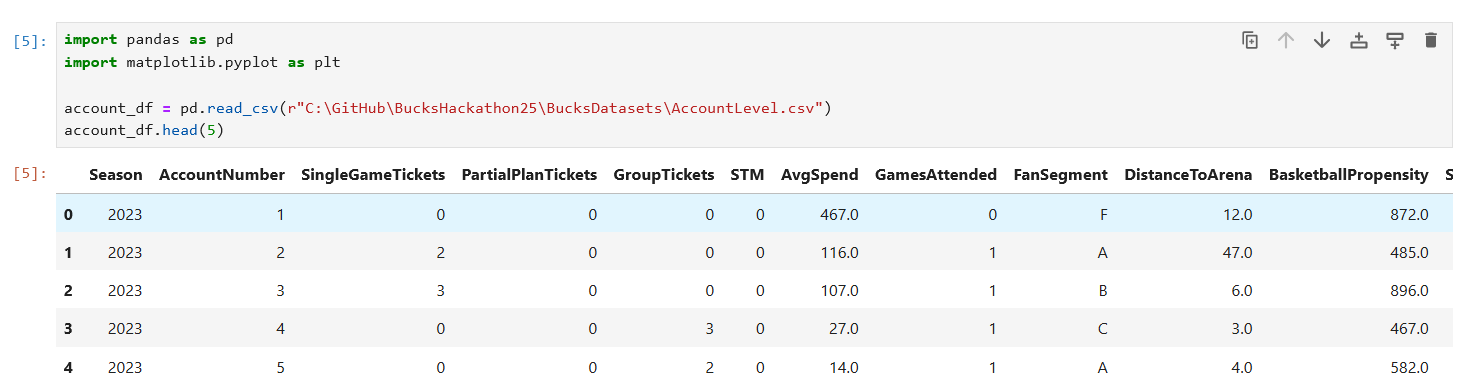
\includegraphics[width=\textwidth]{C:/GitHub/BucksHackathon25/ProjectProposal/images/image_one.png}
    \caption{Loading Up \texttt{AccountLevel}}
\end{figure}

\begin{figure}[h!]
    \centering
    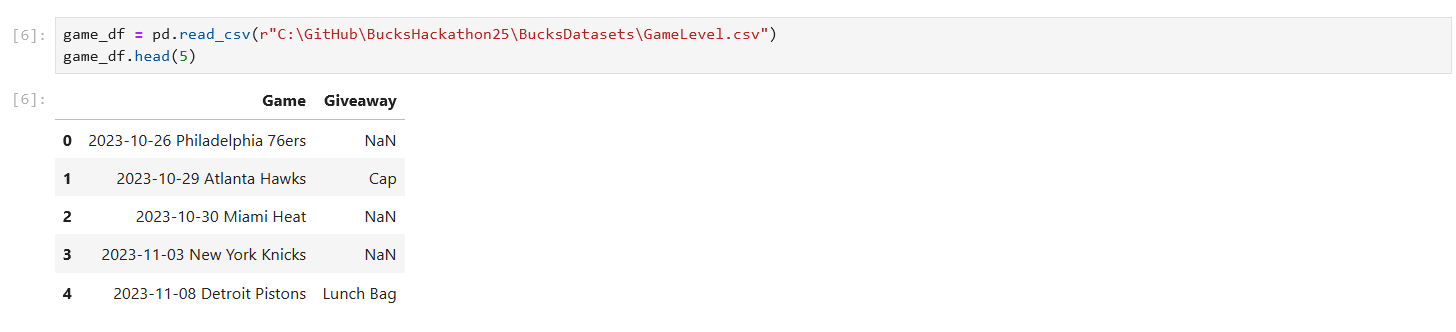
\includegraphics[width=\textwidth]{C:/GitHub/BucksHackathon25/ProjectProposal/images/image_two.png}
    \caption{Loading Up \texttt{GameLevel}}
\end{figure}

\begin{figure}[h!]
    \centering
    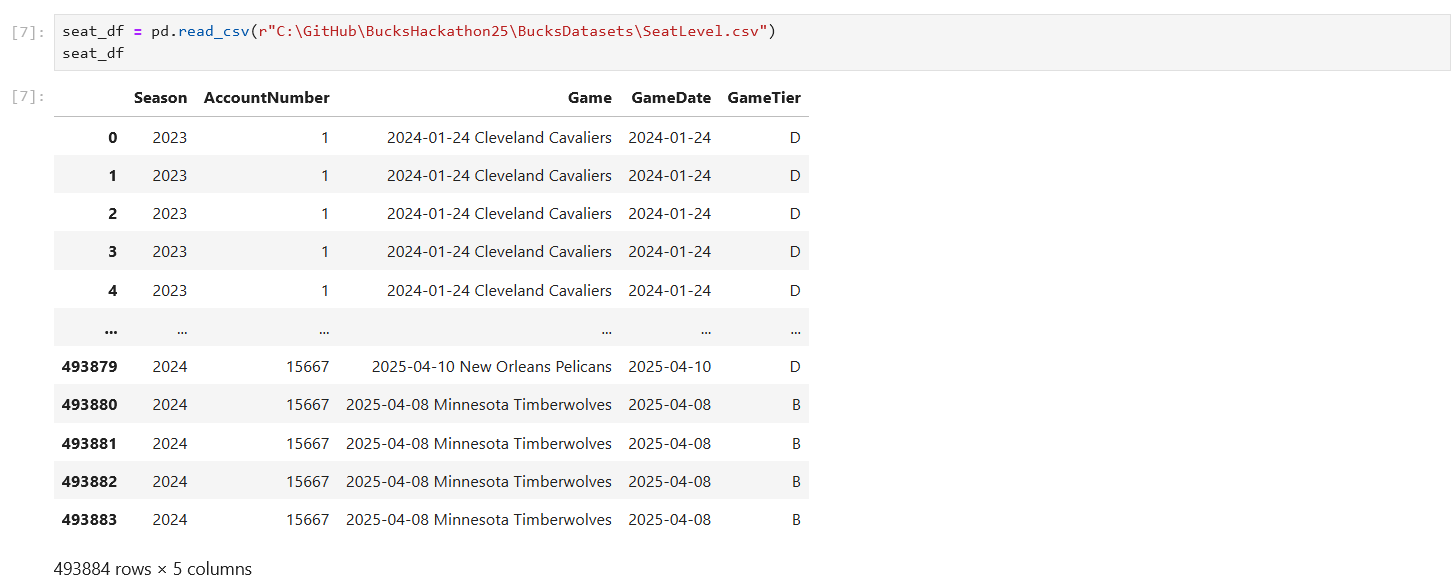
\includegraphics[width=\textwidth]{C:/GitHub/BucksHackathon25/ProjectProposal/images/image_three.png}
    \caption{Loading Up \texttt{SeatLevel}}
\end{figure}
    
\end{document}